\chapter{This is in a Different File With Stuff}
Well well well, what do we have here?. Use this command in the document body to insert the contents of another file named filename.tex; again this file should not contain any LATEX preamble. LATEX will start a new page before processing the material input from filename.tex. Make sure not to include the extension .tex in the filename, as this will stop the file from being input (the extension can optionally be included with input and import). It is not possible to nest include commands. Each file that gets has its own .aux file storing information of created labels and contents for the table of contents, list of figures, etc. You can use  with a comma separated list of file names (make sure that there are no leading or trailing spaces). If you do this LATEX will only process the files contained in that list. This can be used to enhance compilation speed if you're only working on a small part of a bigger document. Page numbers and cross references will however still work, as the .aux files of left out files will still be processed.
\section{Section Title}

\begin{figure}[H] % Use H from the float package so image shows up in the part of text where you put the environment

	\centering
	
\includegraphics[width=5cm]{usd}
	\caption{USD Logo}
\end{figure}

What on earth is this?


\section{Tables Tables Tables}

\begin{table}[h]
	\caption{A table of numbers}
	\begin{center}
		\begin{tabular}{|c|c|c|}
				\hline
			First&Second&Third\\
				\hline
			1&2&3\\
				\hline
		\end{tabular}
	\end{center}
\end{table}

\chapter{Graphs, Quotes, and Citations}
\lipsum[1-2]

\section{Graphs}
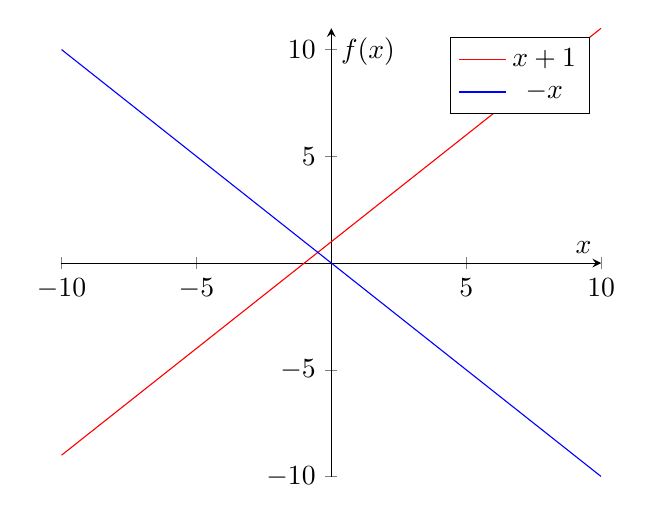
\begin{tikzpicture}
	\begin{axis}[
		axis lines = center,
		xlabel = \(x\),
		ylabel = {\(f(x)\)},
		]
		%Below the red parabola is defined
		\addplot [
		domain=-10:10,
		samples=100,
		color=red,
		]
		{x + 1};
		\addlegendentry{\(x + 1\)}
		%Here the blue parabola is defined
		\addplot [
		domain=-10:10,
		samples=100,
		color=blue,
		]
		{-x};
		\addlegendentry{\(-x\)}

	\end{axis}
\end{tikzpicture}

\section{Block quotes}
This part is an example of making a quote. We'll fill it out with stuff so it becomes more than one line without using lorem ipsum
\begin{quote}
	\lipsum[1-2] \parencite{wombat2016} % Parenthesis citation.
\end{quote}

According to \footcite[Quote from][According to me, this is really neat]{lion2010}, this is something. What can we learn from this exercise? Well, if we add another paragraph, bla bla bla bla bla.

Another example of citation is using this \parencite[see][page 12]{wikibook}

